\documentclass[12pt, a4paper, notitlepage]{report}
\usepackage{mathptmx}
\usepackage[T1]{fontenc}
\usepackage[utf8x]{inputenc}
\usepackage[english]{babel}
\usepackage{graphicx}
\usepackage{float}
\usepackage{amsmath}
\usepackage{mathtools}
\usepackage{amsfonts}
\usepackage{enumerate}
\usepackage{subfigure}
\usepackage[caption = false]{subfig}
\usepackage[top=2.5cm, bottom=2.5cm, left=2cm, right=2cm]{geometry}
\usepackage[font={small,it}]{caption}
\usepackage{fancyhdr}
\usepackage{listings}
\usepackage{color}

\graphicspath{ {./Res\_L5\_k10/} {./Res\_L5\_k100/} {./Res\_L5\_k1000/} {./Res\_L10\_k10/} {./Res\_L10\_k100/} {./Res\_L10\_k1000/} {./Res\_L15\_k10/} {./Res\_L15\_k100/} {./Res\_L15\_k1000/} }

\definecolor{dkgreen}{rgb}{0,0.6,0}
\definecolor{gray}{rgb}{0.5,0.5,0.5}
\definecolor{mauve}{rgb}{0.58,0,0.82}
\definecolor{lyellow}{rgb}{1,1,0.9}

\lstset{backgroundcolor=\color{lyellow},
	frame=tb,
	language=Fortran,
	aboveskip=3mm,
	belowskip=3mm,
	showstringspaces=false,
	columns=flexible,
	basicstyle={\small\ttfamily},
	numbers=none,
	numberstyle=\tiny\color{gray},
	keywordstyle=\color{blue},
	commentstyle=\color{dkgreen},
	stringstyle=\color{mauve},
	breaklines=true,
	breakatwhitespace=true,
	tabsize=3
}

\pagestyle{fancy}
\lhead{Tommaso Tabarelli}
\chead{\thepage}
\rhead{\today}
\cfoot{Information theory and computation}
\rfoot{A.y. 2019/2020}
\lfoot{Exercise 6}

\begin{document}

\begin{center}
	\LARGE{Quantum information and computation: homework 6}\\
	\Large{of Tommaso Tabarelli}
\end{center}


\begin{abstract}
	In this homework we are asked to analyze the results of the analysis of the \textit{unidimensional quantum harmonic oscillator}. In particular we are asked to compare computer eigenvalues and eigenvector results with theoresical ones. We should produce these results using a Fortran program.\\
	To do it we should write the discretize matrix form of the \textit{Hamiltonian} operator $\hat{H}$ act on this representation using \textit{DSYEV} lapack routine, in particular we should compute eigenvalues and eigenvectors.
\end{abstract}

\section*{Theory}
The unidimensional quantum harmonic oscillator is the quantum version of the classic harmonic oscillator in which a particle of mass \textit{m} is attached to an extreme of an ideal spring, this one having the other extreme fixed in the origin.\\
Naming $x$ the spring extension (with respect to the origin), $p$ the particle linear momentum and $k$ the spring constant, the classical system is described by the following equation for the energy:
$$ H = \frac{p^2}{2m} + \frac{1}{2} k x^2 $$

In the quantum case one should use the corresponding operators:

$$ \hat{H} = \frac{\hat{P}^2}{2m} + \frac{1}{2} k \hat{X}^2 $$

and to find the energies, the eigenvalues problem to solve is:

$$ \hat{H} \vert \psi_E \rangle = E \vert \psi_E \rangle $$

The problem now is that we want to write $\hat{H}$ in a matrix form to analyze it. To do it a representation form has to be chosen. We shall use the x-representation for both $ \vert \psi \rangle $ and $ \hat{H} $. In this representation we have:

$$ \hat{P} = -i \hbar \frac{ \partial }{ \partial x} \qquad \hat{X} = x \qquad  $$

So the $\hat{H}$ eigenvalues equation in this representation becomes (using also $\omega = \sqrt{k/m}$):

$$ - \frac{\hbar^2}{2m} \frac{\partial^2 }{ \partial x^2} \psi_E (x)+ \frac{1}{2} m \omega^2 x^2 \psi_E (x) = E \psi_E (x) $$

It can be shown that the eigenvalues are:

$$ E_n = \hbar \omega \left( n + \frac{1}{2} \right) \quad n=0,1,2,... $$

and the eigenfunctions are (in x-representation):

$$ \psi_n (x) = \frac{1}{\sqrt{n! 2^n}} \left( \frac{m \omega}{\pi \hbar} \right)^{1/4} H_n(\xi) e^{-\frac{\xi^2}{2}} \qquad \xi = \sqrt{\frac{m \omega}{\hbar}} x $$

where $ H_n(\xi) $ are the \textit{Hermite polynomials} of order $n$.

Since in a computer continuos variable can not be represented, to write down the matrix form of the matrix one has to fix a discretization. The only thing to discretize is the second order derivative, which has the form (naming $h$ the discretization spacing):

$$ \frac{\partial^2 }{ \partial x^2} f(x) \simeq \frac{f(x-h) -2f(x) + f(x+h))}{h^2} $$

Naming $x_i$ the points of the interval, we have that $x_i \pm h =  x_{i \pm 1}$. Thus the discretized Hamiltonian has the form:

$$ H = \left( \begin{matrix}
	\frac{2 \hbar^2}{2m h^2} + \frac{1}{2} m \omega^2 x^2 & -\frac{\hbar^2}{2m h^2} & 0 & \dots & & & 0 \\
	-\frac{\hbar^2}{2m h^2} & \frac{2 \hbar^2}{2m h^2} + \frac{1}{2} m \omega^2 x^2 & -\frac{\hbar^2}{2m h^2} & 0 & & \dots & \vdots \\
	0 & -\frac{\hbar^2}{2m h^2} & \frac{2 \hbar^2}{2m h^2} + \frac{1}{2} m \omega^2 x^2 & -\frac{\hbar^2}{2m h^2} & 0 & \dots & \\
	\vdots & \ddots & \ddots & \ddots  & \ddots & \ddots & \dots & \\
	0 & & \dots &  & 0 & -\frac{\hbar^2}{2m h^2} & \frac{2 \hbar^2}{2m h^2} + \frac{1}{2} m \omega^2 x^2 \\
\end{matrix} \right) $$

\section*{Code development}
The Fortran program first reads 2 files in which the size of the interval and the number of intervals to use for the discretization are written. Then variables are allocated. After that, the proper evaluation takes place: basing on the number of points, a proper Hamiltonian is created and it is used to feed lapack's \textit{DSYEV} subroutine after having let it found the optimal dimension to work with. Increasing order eigenvalues are collected and stored. The Hamiltonian is changed: after the subroutine call it contains the "normalized" eigenvectors. It is important to notice that these eigenvectors are not properly normalized: by construction they represent the eigenfunctions evaluated in the points of the considered interval. \textit{DSYEV} normalizes the norm of them, thus it does:
$$ \lVert \phi(x) \rVert = 1 \quad \Rightarrow \quad \sqrt{\sum\limits_i \phi(x_i)^2} = 1 \quad \Rightarrow \quad \sum\limits_i  \left( \phi(x_i) \cdot 1 \right)^2 = 1 $$

where it is emphasized the fact that this normalization is similar to ask that the integral of the squared function is 1 using all \textit{size-1} intervals.\\
What we want is instead:
$$ \int\limits_{-\infty}^{+\infty} \Vert \psi \Vert^2 dx = 1 \quad \overset{\text{discretizing}}{\Rightarrow} \quad \sum\limits_i  \left( \psi(x_i)^2 \cdot h_i \right) = 1 \quad \Rightarrow \quad \sum\limits_i  \left( \psi(x_i) \cdot \sqrt{h_i} \right)^2 = 1 $$

It is immediate now to see that to get the properly normalized eigenfunction one has to divide the \textit{DSYEV} eigenvectors by $\sqrt{h}$ where h is the common spacing, i.e. the size of the discretization interval:
$$ \psi(x_i) = \frac{\phi(x_i)}{\sqrt{h}} $$

Theoretical eigenfunctions are also evaluated: to do it, 2 modules are defined. The first is used to evaluate Hermite polynomials while the second is used to evaluate the factorial value of a number.
All results are stored to proper files.

To execute a better task and explore different parameters values a python script was implement, acting on different interval sizes and number of points. This script also creates proper folders in which store the data, saving current date and time as folder name.

The python script also takes care to plot eigenvalues results and compare the first 10 (arbitrary value choice to try to limitate memory issues) approximated and theoretical eigenfunctions.



\section*{Results}

\begin{figure*}[h!]
	\centering
	\subfigure[Number points = 11]{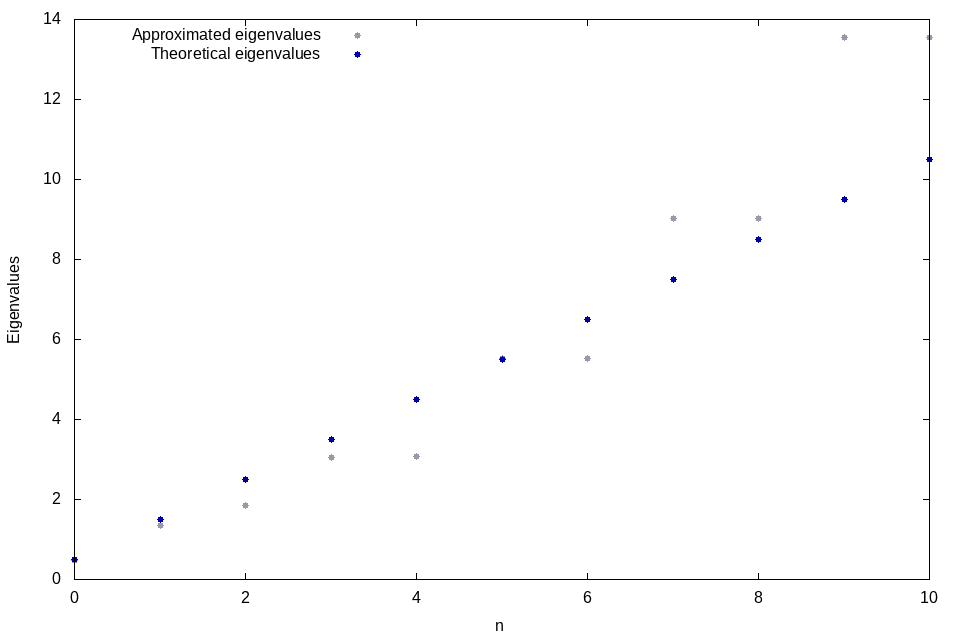
\includegraphics[scale=0.25]{./Res_L5_k10/eig_plot.png}}\label{L5k10}
	\subfigure[Number points = 101]{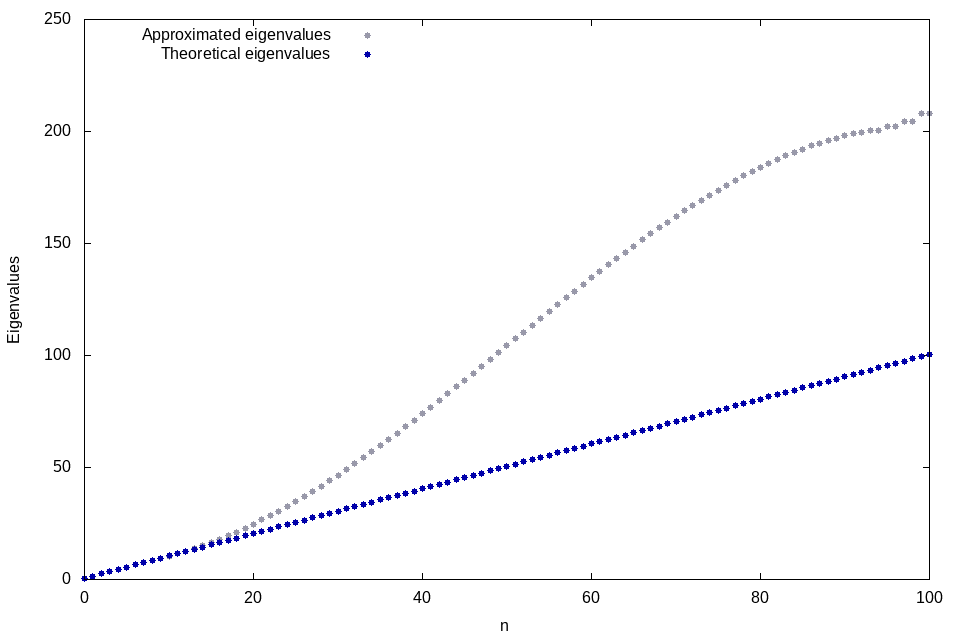
\includegraphics[scale=0.25]{./Res_L5_k100/eig_plot.png}}\label{L5k100}
	\subfigure[Number points = 1001]{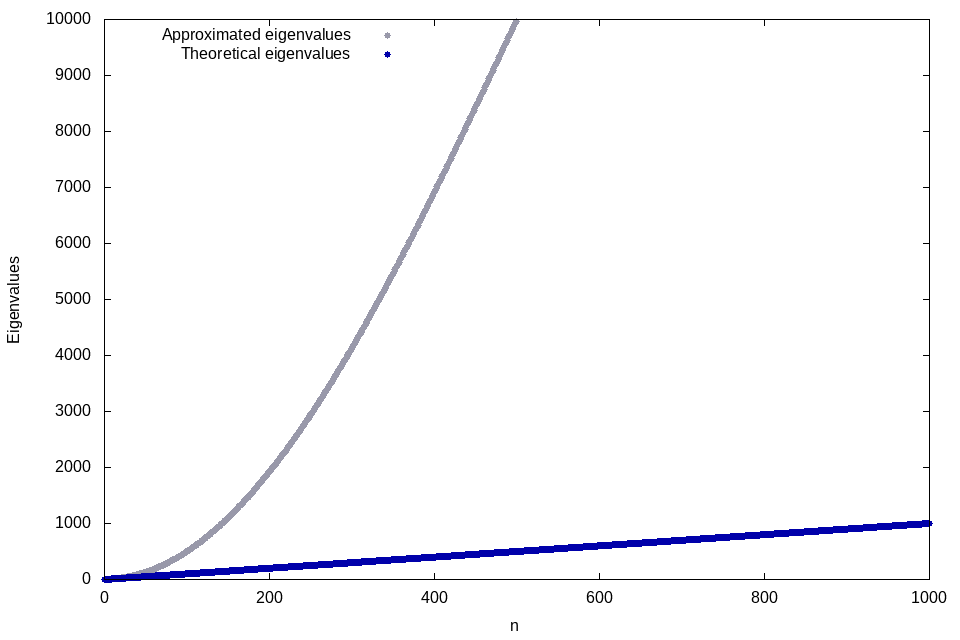
\includegraphics[scale=0.25]{./Res_L5_k1000/eig_plot.png}}\label{L5k1000}
	\subfigure[Number points = 10001]{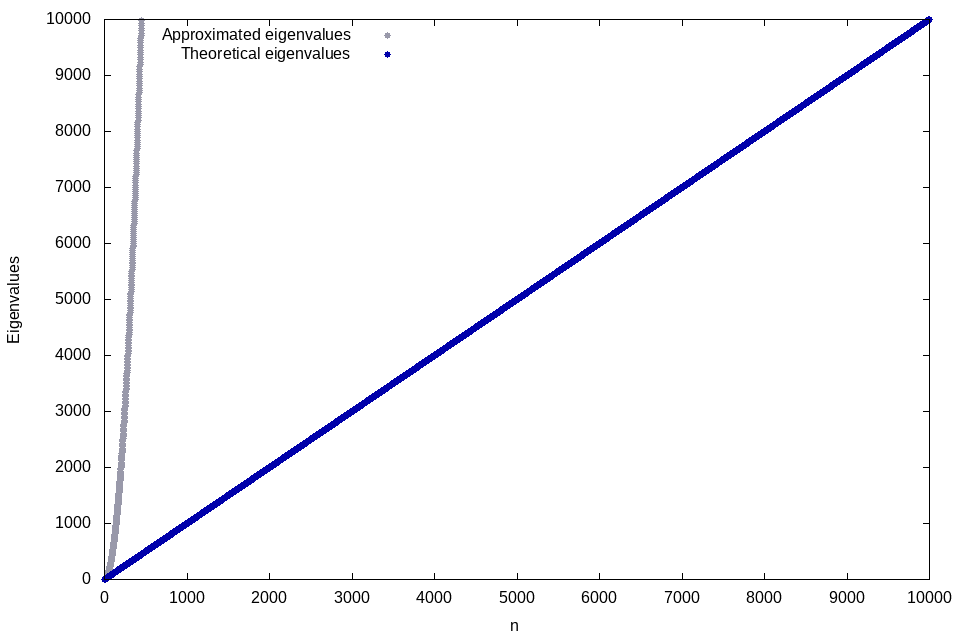
\includegraphics[scale=0.25]{./Res_L5_k10000/eig_plot.png}}\label{L5k10000}
	\caption{Eigenvalues evaluated using the interval [-5,5]}
\end{figure*}

\begin{figure*}[h!]
	\centering
	\subfigure[Number points = 11]{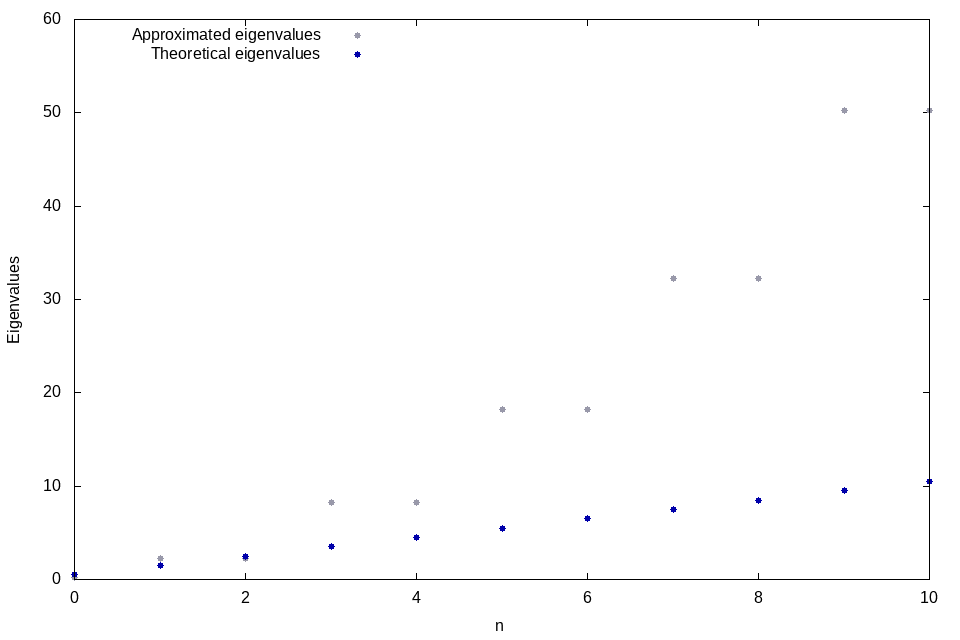
\includegraphics[scale=0.25]{./Res_L10_k10/eig_plot.png}}\label{L10k10}
	\subfigure[Number points = 101]{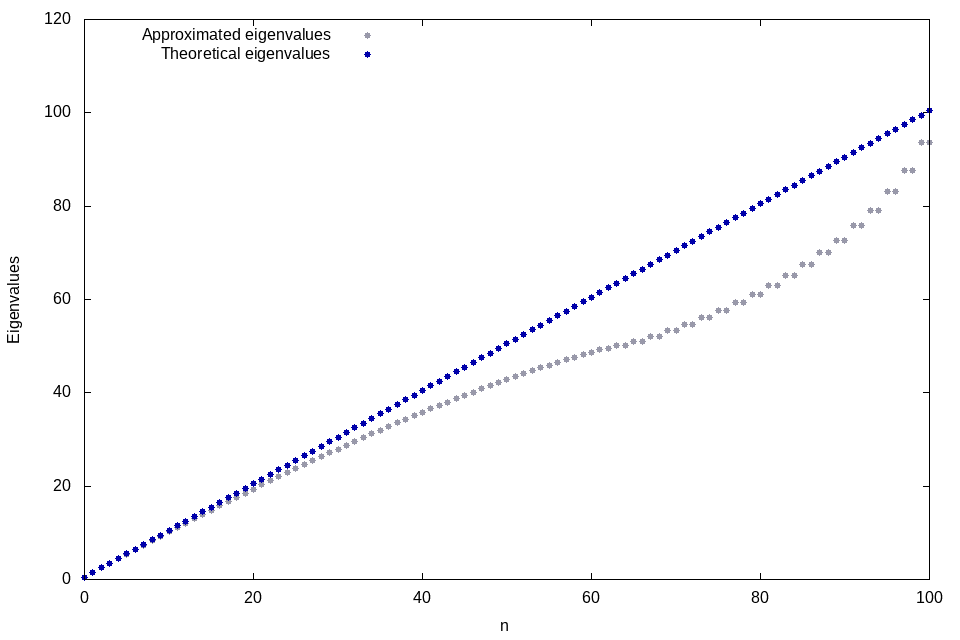
\includegraphics[scale=0.25]{./Res_L10_k100/eig_plot.png}}\label{L10k100}
	\subfigure[Number points = 1001]{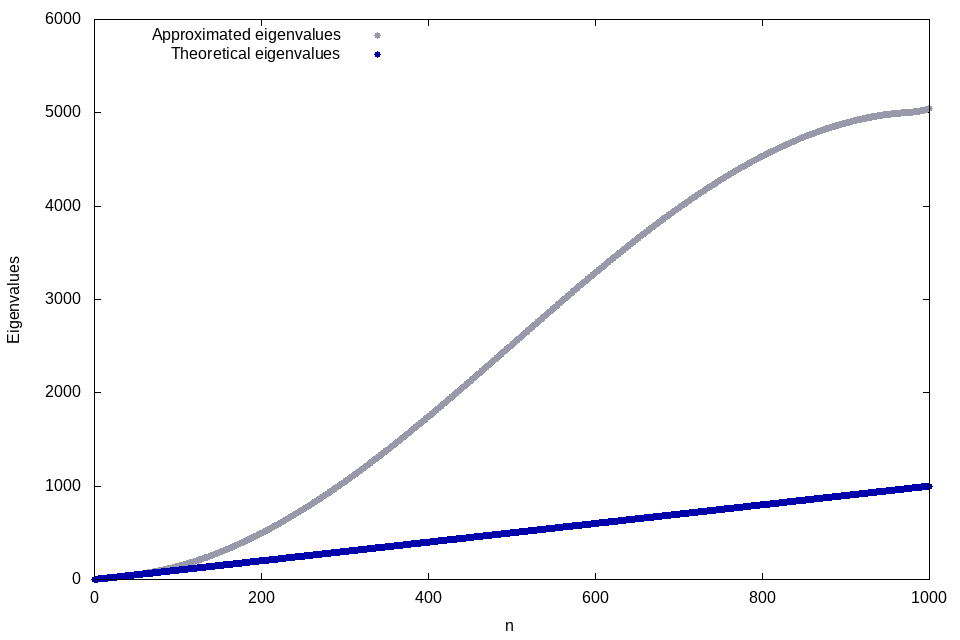
\includegraphics[scale=0.25]{./Res_L10_k1000/eig_plot.png}}\label{L10k1000}
	\subfigure[Number points = 10001]{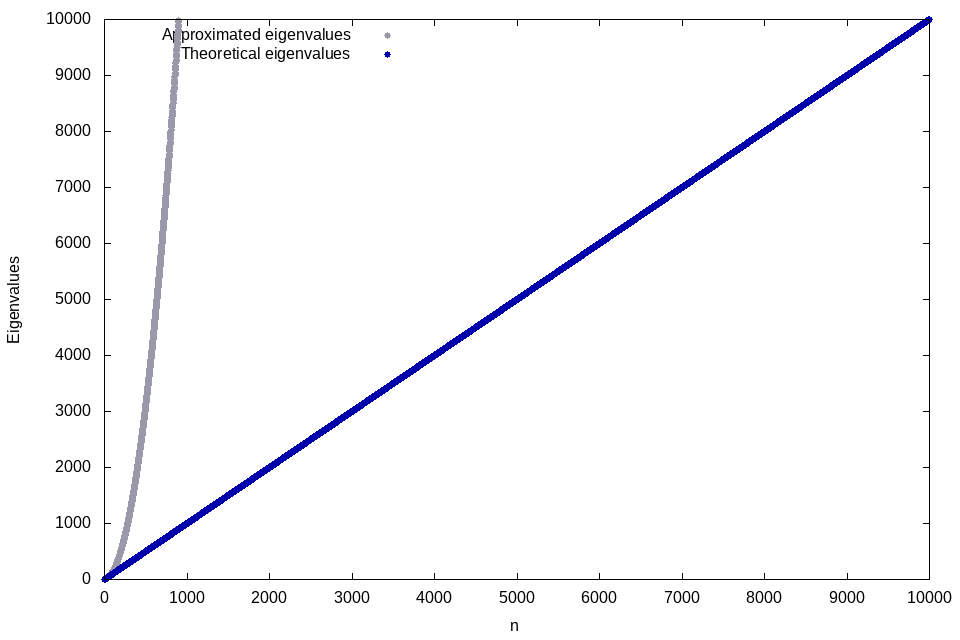
\includegraphics[scale=0.25]{./Res_L10_k10000/eig_plot.png}}\label{L10k10000}
	\caption{Eigenvalues evaluated using the interval [-10,10]}	
\end{figure*}

\begin{figure*}[h!]
	\centering
	\subfigure[Number points = 11]{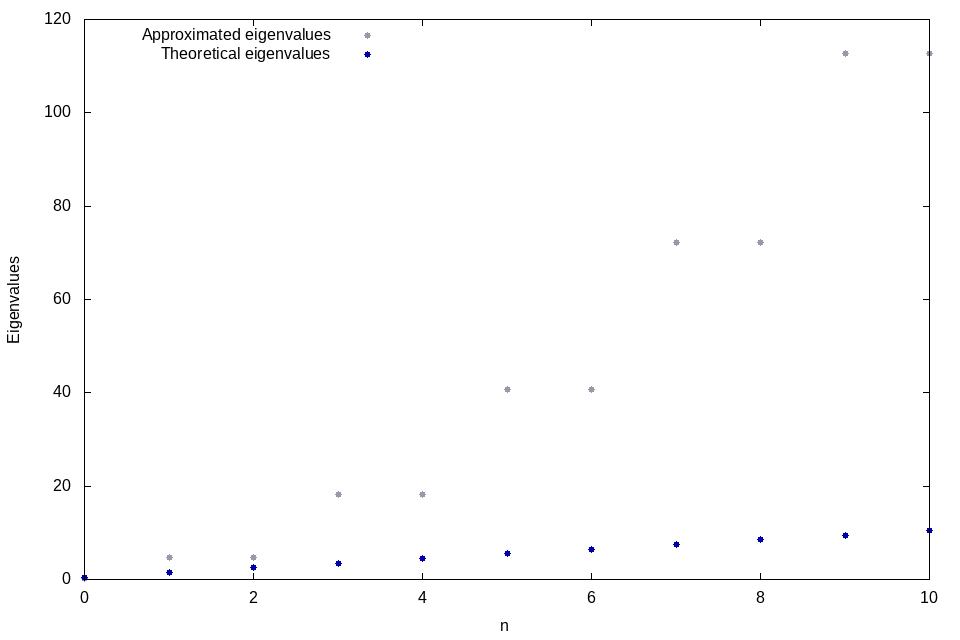
\includegraphics[scale=0.25]{./Res_L15_k10/eig_plot.png}}\label{L15k10}
	\subfigure[Number points = 101]{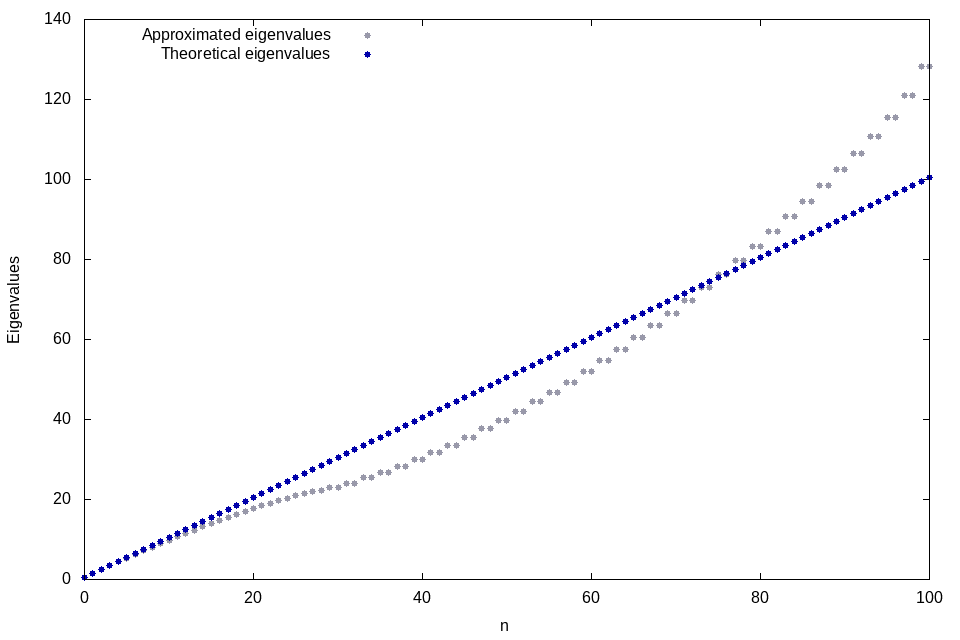
\includegraphics[scale=0.25]{./Res_L15_k100/eig_plot.png}}\label{L15k100}
	\subfigure[Number points = 1001]{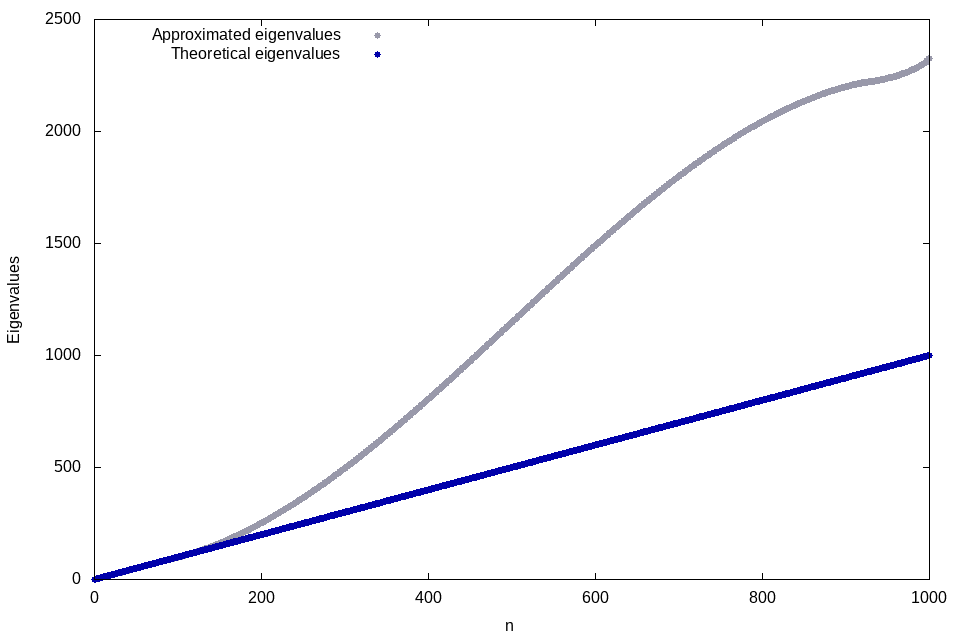
\includegraphics[scale=0.25]{./Res_L15_k1000/eig_plot.png}}\label{L15k1000}
	\subfigure[Number points = 10001]{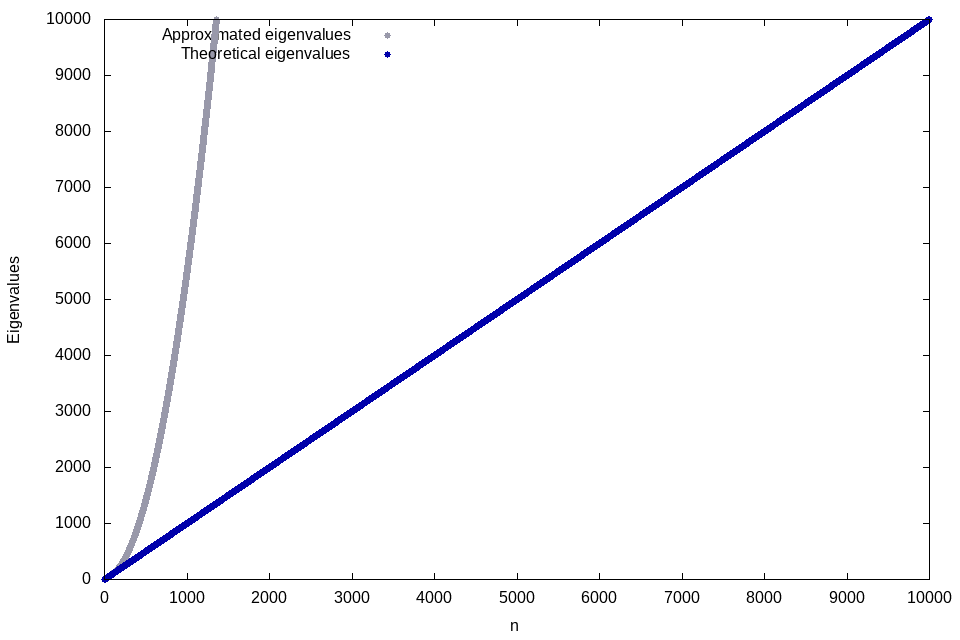
\includegraphics[scale=0.25]{./Res_L15_k10000/eig_plot.png}}\label{L15k10000}
	\caption{Eigenvalues evaluated using the interval [-15,15]}
\end{figure*}

The images show that the discretization plays an important role in determining the eigenvalues approximations. Indeed increasing the number of points in the interval leads to a better discretization untill a certain threshold, which is around 100; after that, the first eigenvalues are still approximated correctly, but the successive ones have a divergent behaviour and can not be considered correct (the eigenvalues are not even written to the file due to their dimension not being compatible with the Fortran format chosen; this has been fixed but the program has not been run again due to time issues). The divergent behaviour is due to the fact that a finite interval is used to evaluate the approximations: the (implicit) boundaries conditions are that the function $\psi$ is 0 out of the interval, causing the potential to become an infinite well and the eigenvalues to follow the corresponding quadratic behaviour (which starts after a certain point) and to have degeneration factor equal to 2 (as can be noticed well in the Figure 2a and 2b).\\

Now, to see if the first eigenvalues are "correct" we shall see if the eigenvectors match the theoretical ones. To do this, the choice was to compare the first ten eigenvectors (manipulated as explained above) and the first ten theoretical eigenfuntcions. The reported results are those of the $n=9$ eigenvector for L=5 and different k (Figure 4).

\begin{figure*}[h!]
	\centering
	\subfigure[Eigenfuntcion: n = 9]{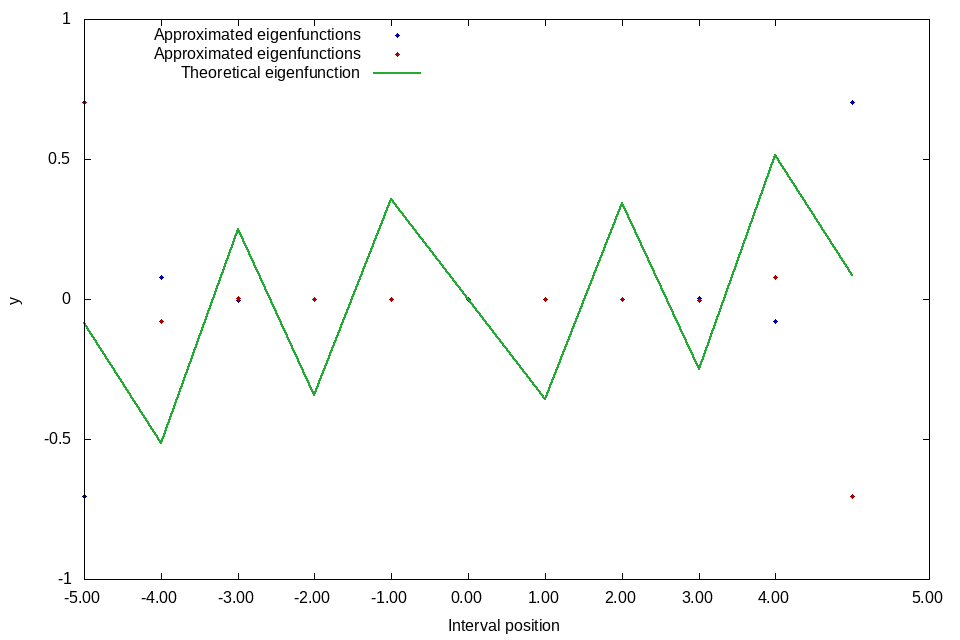
\includegraphics[scale=0.25]{./Res_L5_k10/eigf9_L5,0_k10.png}}\label{L5k10}
	\subfigure[Eigenfuntcion: n = 9]{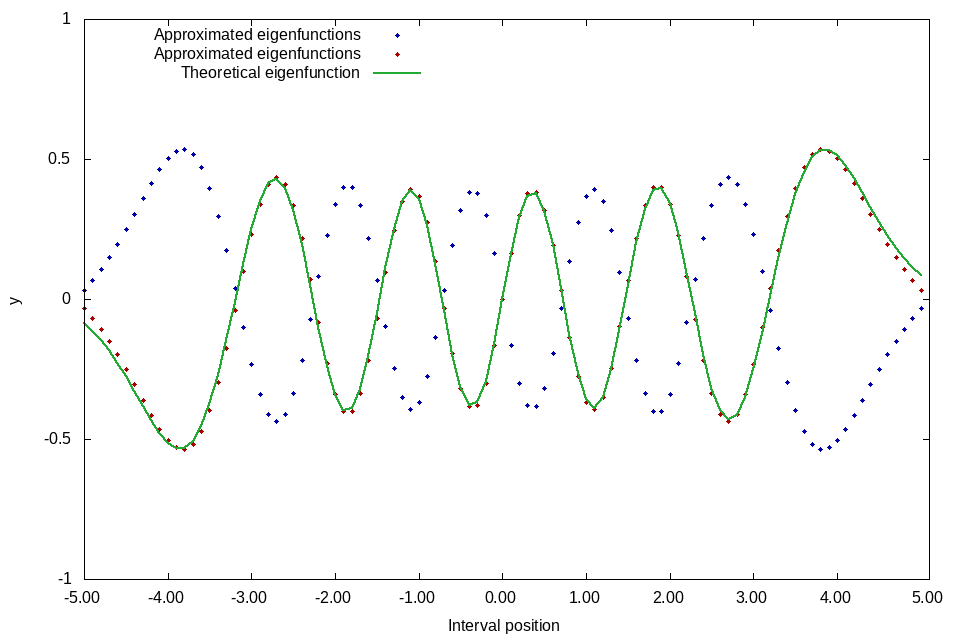
\includegraphics[scale=0.25]{./Res_L5_k100/eigf9_L5,0_k100.png}}\label{L5k10}
	\subfigure[Eigenfuntcion: n = 9]{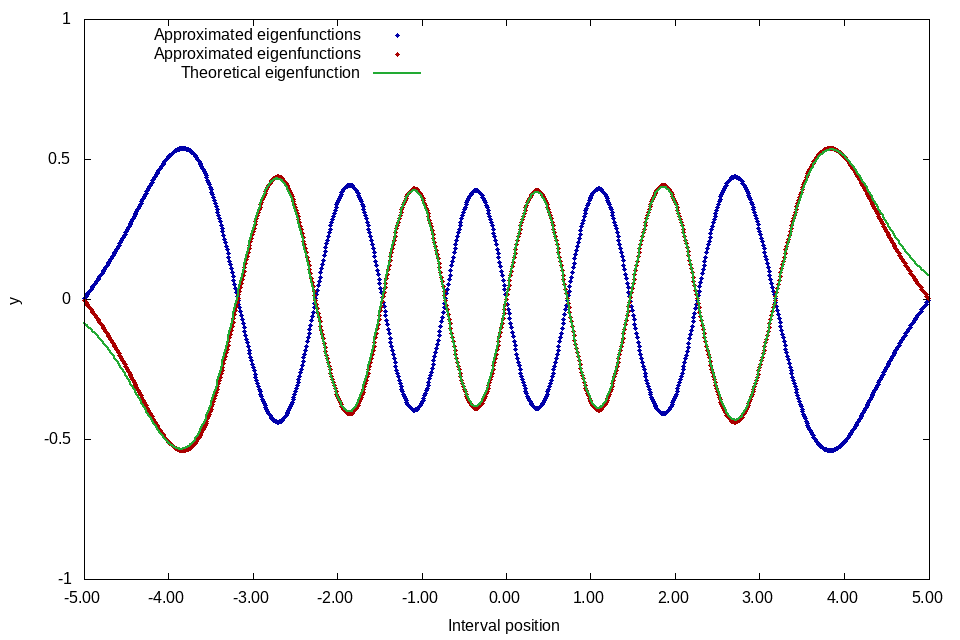
\includegraphics[scale=0.25]{./Res_L5_k1000/eigf9_L5,0_k1000.png}}\label{L5k10}
	\subfigure[Eigenfuntcion: n = 9]{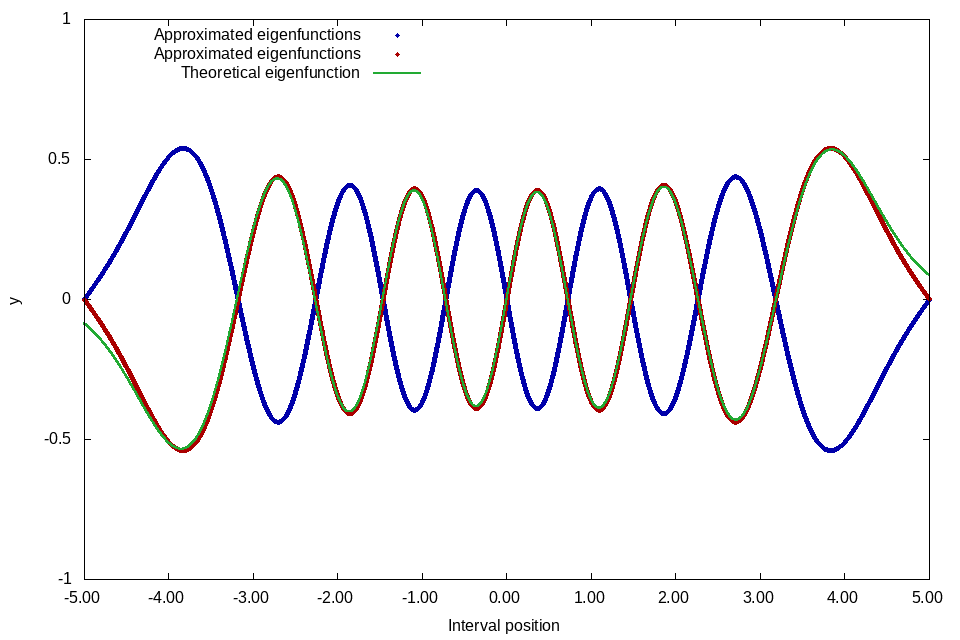
\includegraphics[scale=0.25]{./Res_L5_k10000/eigf9_L5,0_k10000.png}}\label{L5k10}
	\caption{Eigenvectors evaluated using the interval [-5,5] using 10 points.}
\end{figure*}

As one can notice, the \textit{boundaries effect} (in the Hamiltonian discretization) also affect the function evaluation over the points outside the interval, which are considered 0 (indeed they do not appear in the discretization). This leads to a bad approximation near the interval extrema. To try to fix it one can chose a larger interval; using the L=15 indeed leads to better results (but of course this does not fix the eigenvalues problem aforementioned).

\begin{figure*}[h!]
	\centering
	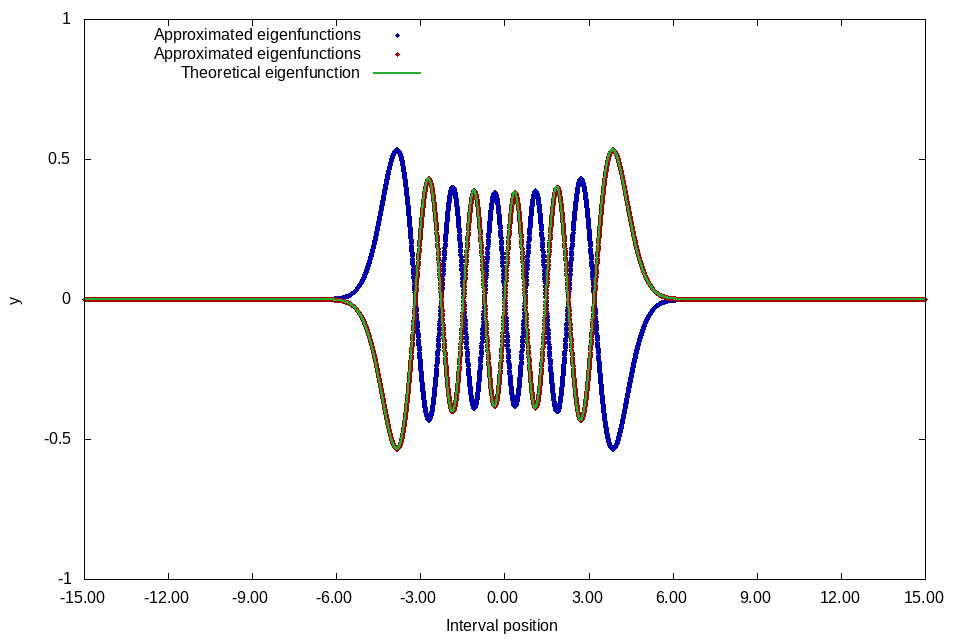
\includegraphics[scale=0.5]{./Res_L15_k10000/eigf9_L15,0_k10000.png}
	\caption{Eigenvectors with n=9 evaluated using the interval [-15,15] using 10000 points.}
\end{figure*}

\section*{Self-evaluation}
In this task I learned how to discretize and properly write in a program the Hamiltonian operator in the x-representation. I also learned how to get approximated eigenvectors and how manipulate them in a proper way to compare them with theoretical ones. Another important thing was to learn how to write down properly normalized \textit{harmonic oscillator} eigenfuntcions; to do it I had to implement a \textit{factorial} subroutine and a \textit{Hermite polynomial} subroutine.\\
For what concerns \textit{Correctness, Stability, Accurate discretization, Flexibility, Efficiency} the considerations are the following.\\

\subsection*{Correctness}

My program does what is expected to do. Some checks are made both in Python script and in Fortran program (for example dimensions are tested to be greater than 0).\\
There are no compilation problems neither memory allocation issues (a special flag is used to compile in order to check for memory error runtime).\\
Pre- and post-conditions and checkpoints are used for the matrix H, but they are implemented manually and are not used very much in the program due to the large amount of time they require to be implemented (compared to the time we have to do the task).


\subsection*{Stability}

In the program \textit{IMPLICIT NONE} is used to avoid strange behaviours due to the implicit type of the variables.\\
Loops are made only on integers (usually the extreme values of the loop variables are the same used to initialize the dimension of the objects).\\
Differences between big numbers are not evaluated in the program to avoid the problem of having finite precision.

\subsection*{Accurate discretization}

As mentioned before, a python script was used to explore different interval width. Using too large intervals the results are bad (as one can see in the 11 points approximations), while using too many points rises memory and time problems (evaluations for 10001 points lasted about 30 min each and eigenvectors file size were about 1.3 GB each).

\subsection*{Flexibility}

I tried to comment as much as possible the code so to have a clear and understandable code.

\subsection*{Efficiency}

I did not implemented the diagonalization of the matrix; instead  \textit{DSYEV} lapack subroutine was used. To evaluate factorial and Hermite polynomials two subroutines were written, but they are quite simple and I think there can be slightly improvements to them.\\
For what concerns memory and time usage, they depend on the parameters passed. Also, time scales with input size (i.e. dimensions of the matrix) as ~$O(n^3)$, so for very high dimension it can take a lot of time to end the task. \\ \\

My work can be improved in different ways: first of all, other parameters can be taken as input in Fortran program (for example, mass and $\omega$); then, to compare eigenfunctions it would be good looking for the eigenfunctions of "uncorrect" eigenvalues, such as those starting from the half of the eigenvalues list (say, starting from ~k/2 index).\\
Other improvements in the data analysis would be to evaluate the infitite well potential eigenvalues and eigenfunctions and compare them with the theoretical ones.



\end{document}